%!TEX root = ../main.tex

\chapter{Kravspecifikation}

\RevisionsTabel{Kravspecifikation}{
Alle	& 1	 	& 23-02-2015  \\
Alle	& 2		& 19-04-2015  \\
Alle	& 3		& 05-15-2015  \\
		& 	 	&   \\
}

%Aktører
\section{Aktører}
%!TEX root = ../../main.tex

I dette afsnit beskrives aktører og deres rolle i systemet. I figur \ref{photo:Aktor} ses aktørdiagram, som beskriver alle aktører og deres forhold til systemet


\begin{figure}[H]
	\centering
	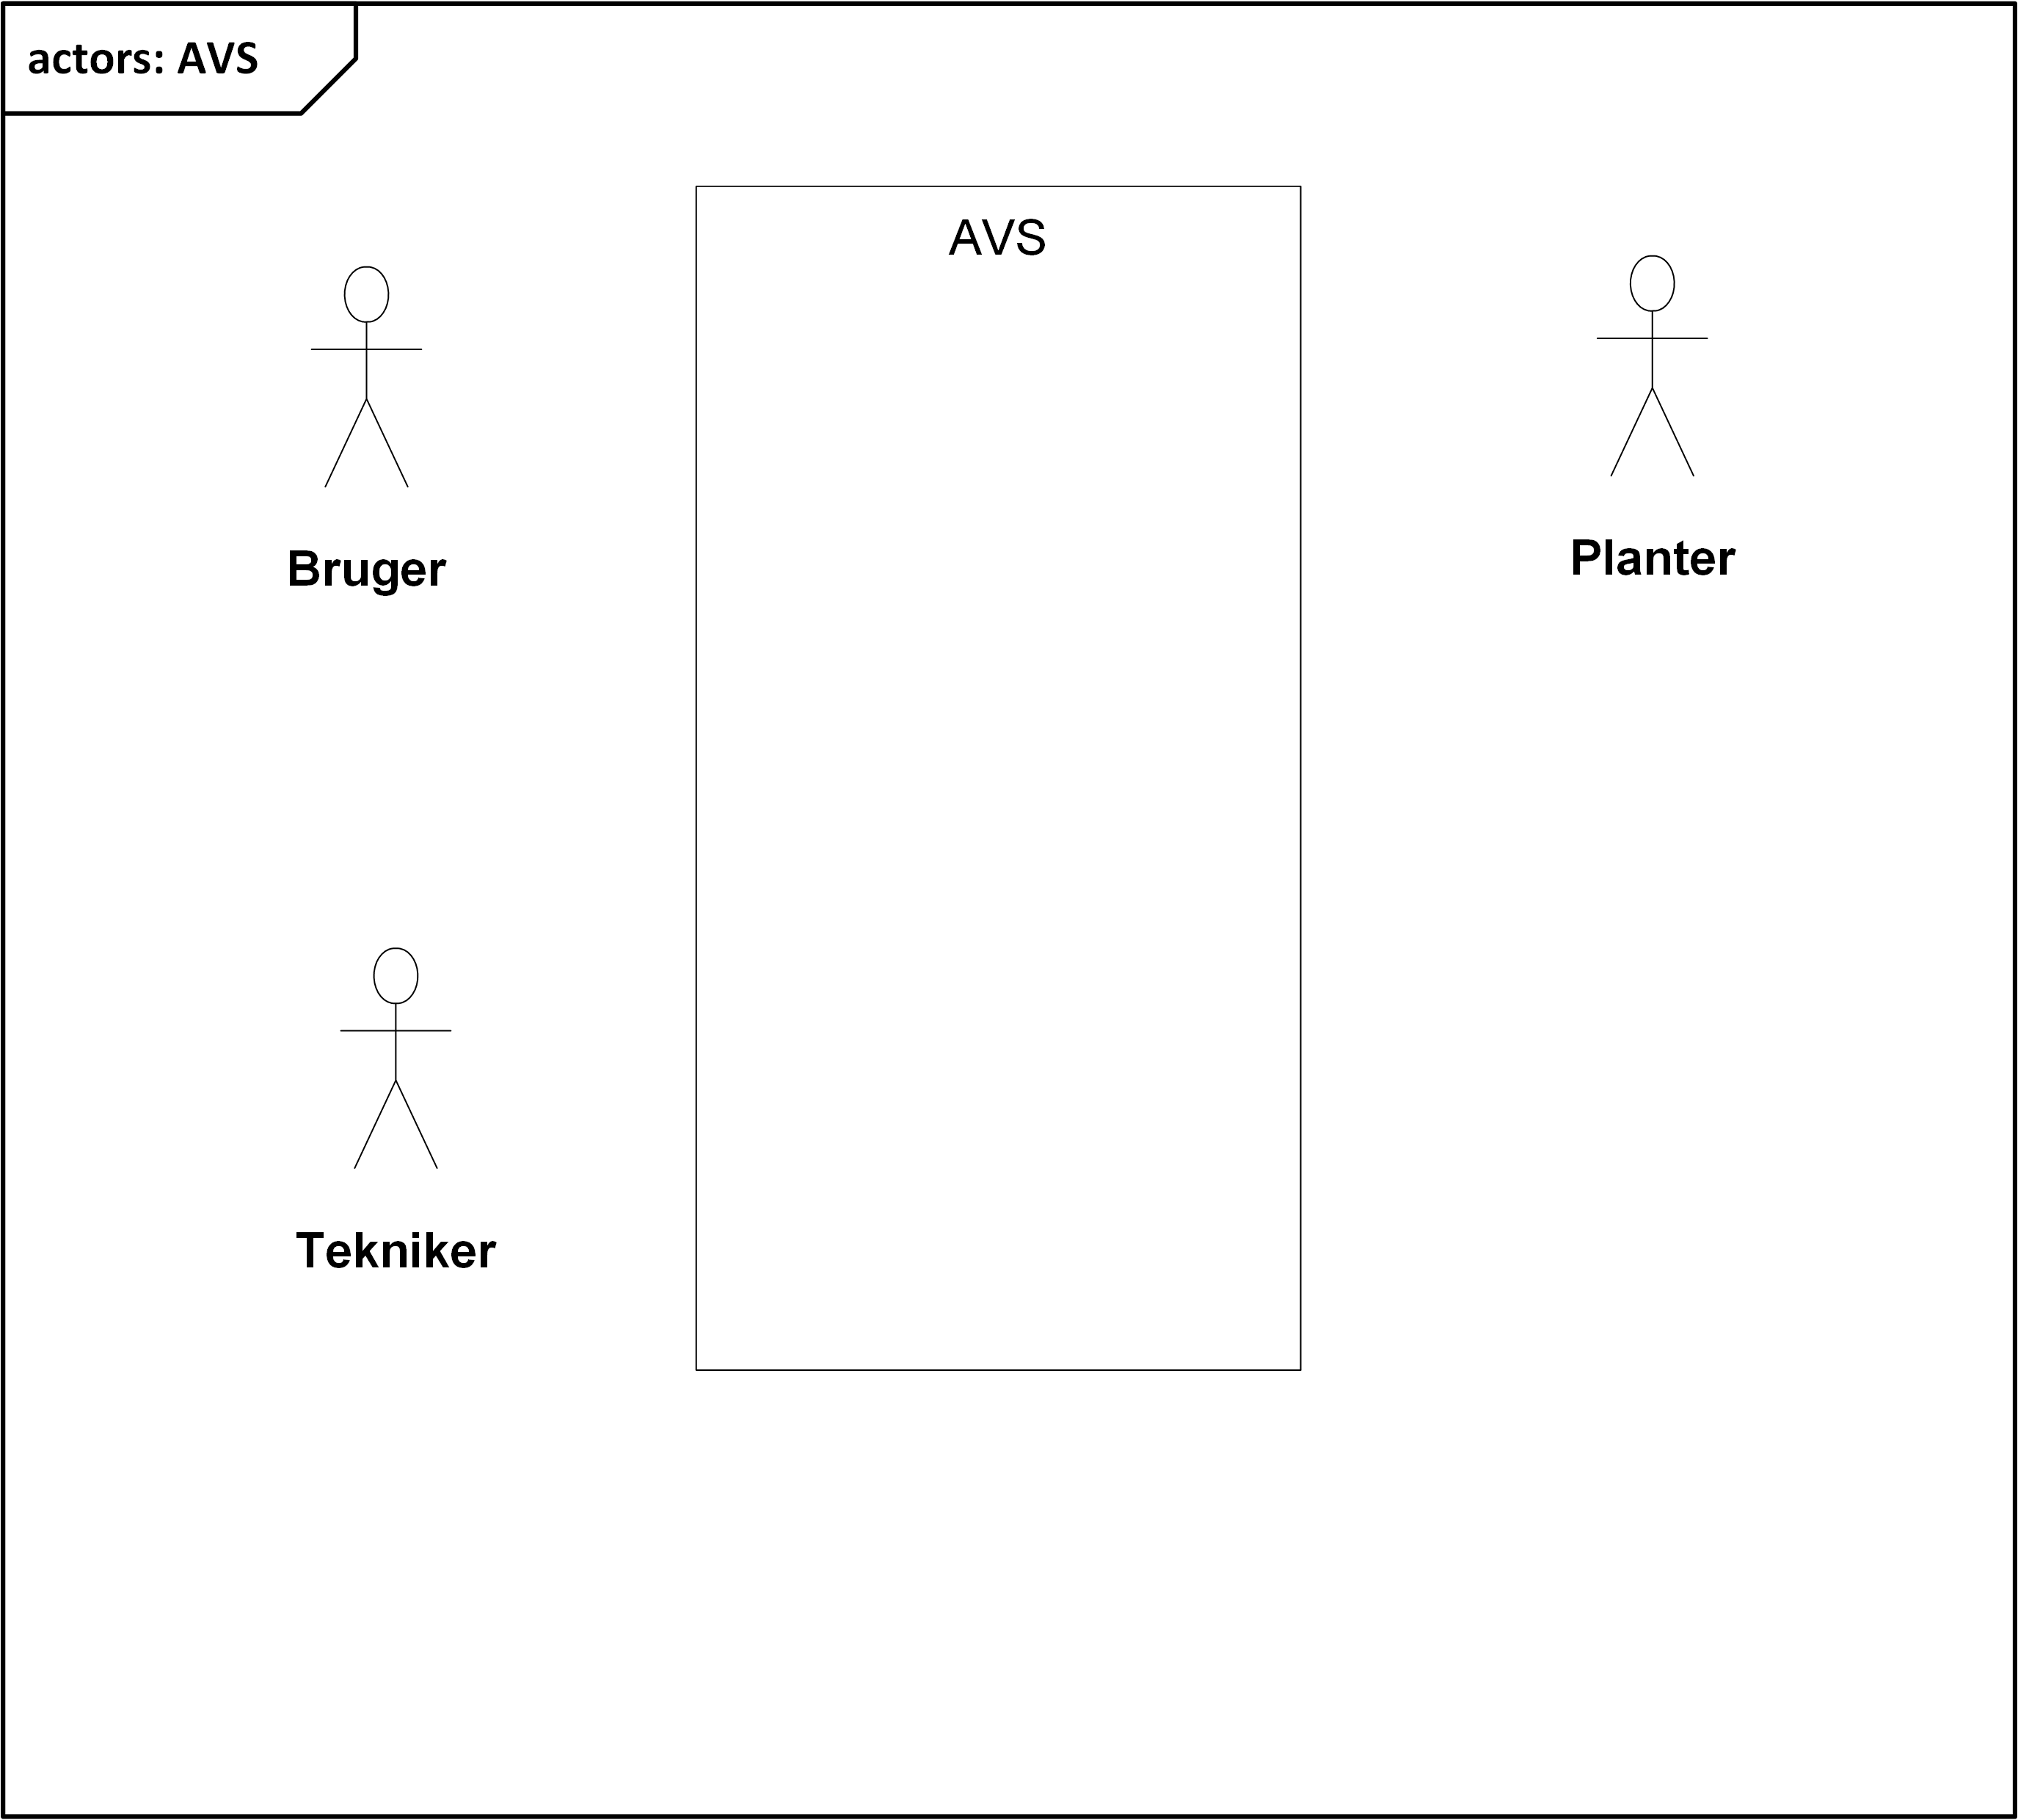
\includegraphics[scale=1]{Kravspecifikation/Actor/Photo/AVS_Actors}
	\caption{AVS Aktører}
	\label{photo:Aktor}
\end{figure}

\newpage

\subsection{Bruger}
\begin{usecase}
\addtitle{Aktørnavn}{Bruger} 
\addfield{type:}{Primær}
\addfield{Beskrivelse:}{Bruger er ham, som til dagligt tilgår systemet. Han ved hvor meget gødning og fugtighed planterne skal have, og angiver disse værdier i brugergrænsefladen. Det er brugeren som løbende ændrer værdierne, så systemet hele tiden er opdateret med værdier der passer til planternes vækststadier.}
\end{usecase}

\subsection{Tekniker}
\begin{usecase}
\addtitle{Aktørnavn}{Tekniker} 
\addfield{type:}{Primær}
\addfield{Beskrivelse:}{Tekniker er en specielt uddannet person. Han har den nødvendige viden om systemet til at kunne installere systemet fra opstart, opsætte nye vandkar mv. En Bruger kan også være tekniker.}
\end{usecase}






%Use Cases
\newpage
\section{Use Cases}
%	Indledning
I dette afsnit ses de forskellige Use Cases. På billede \ref{photo:UseCD} ses et Use case diagram, som viser en simpel repræsentation af bruger, tekniker og \glslink{plante}{planters} interaktion med systemet og en afbildning af de forskellig Use Cases. 



\begin{figure}[H]
	\centering
	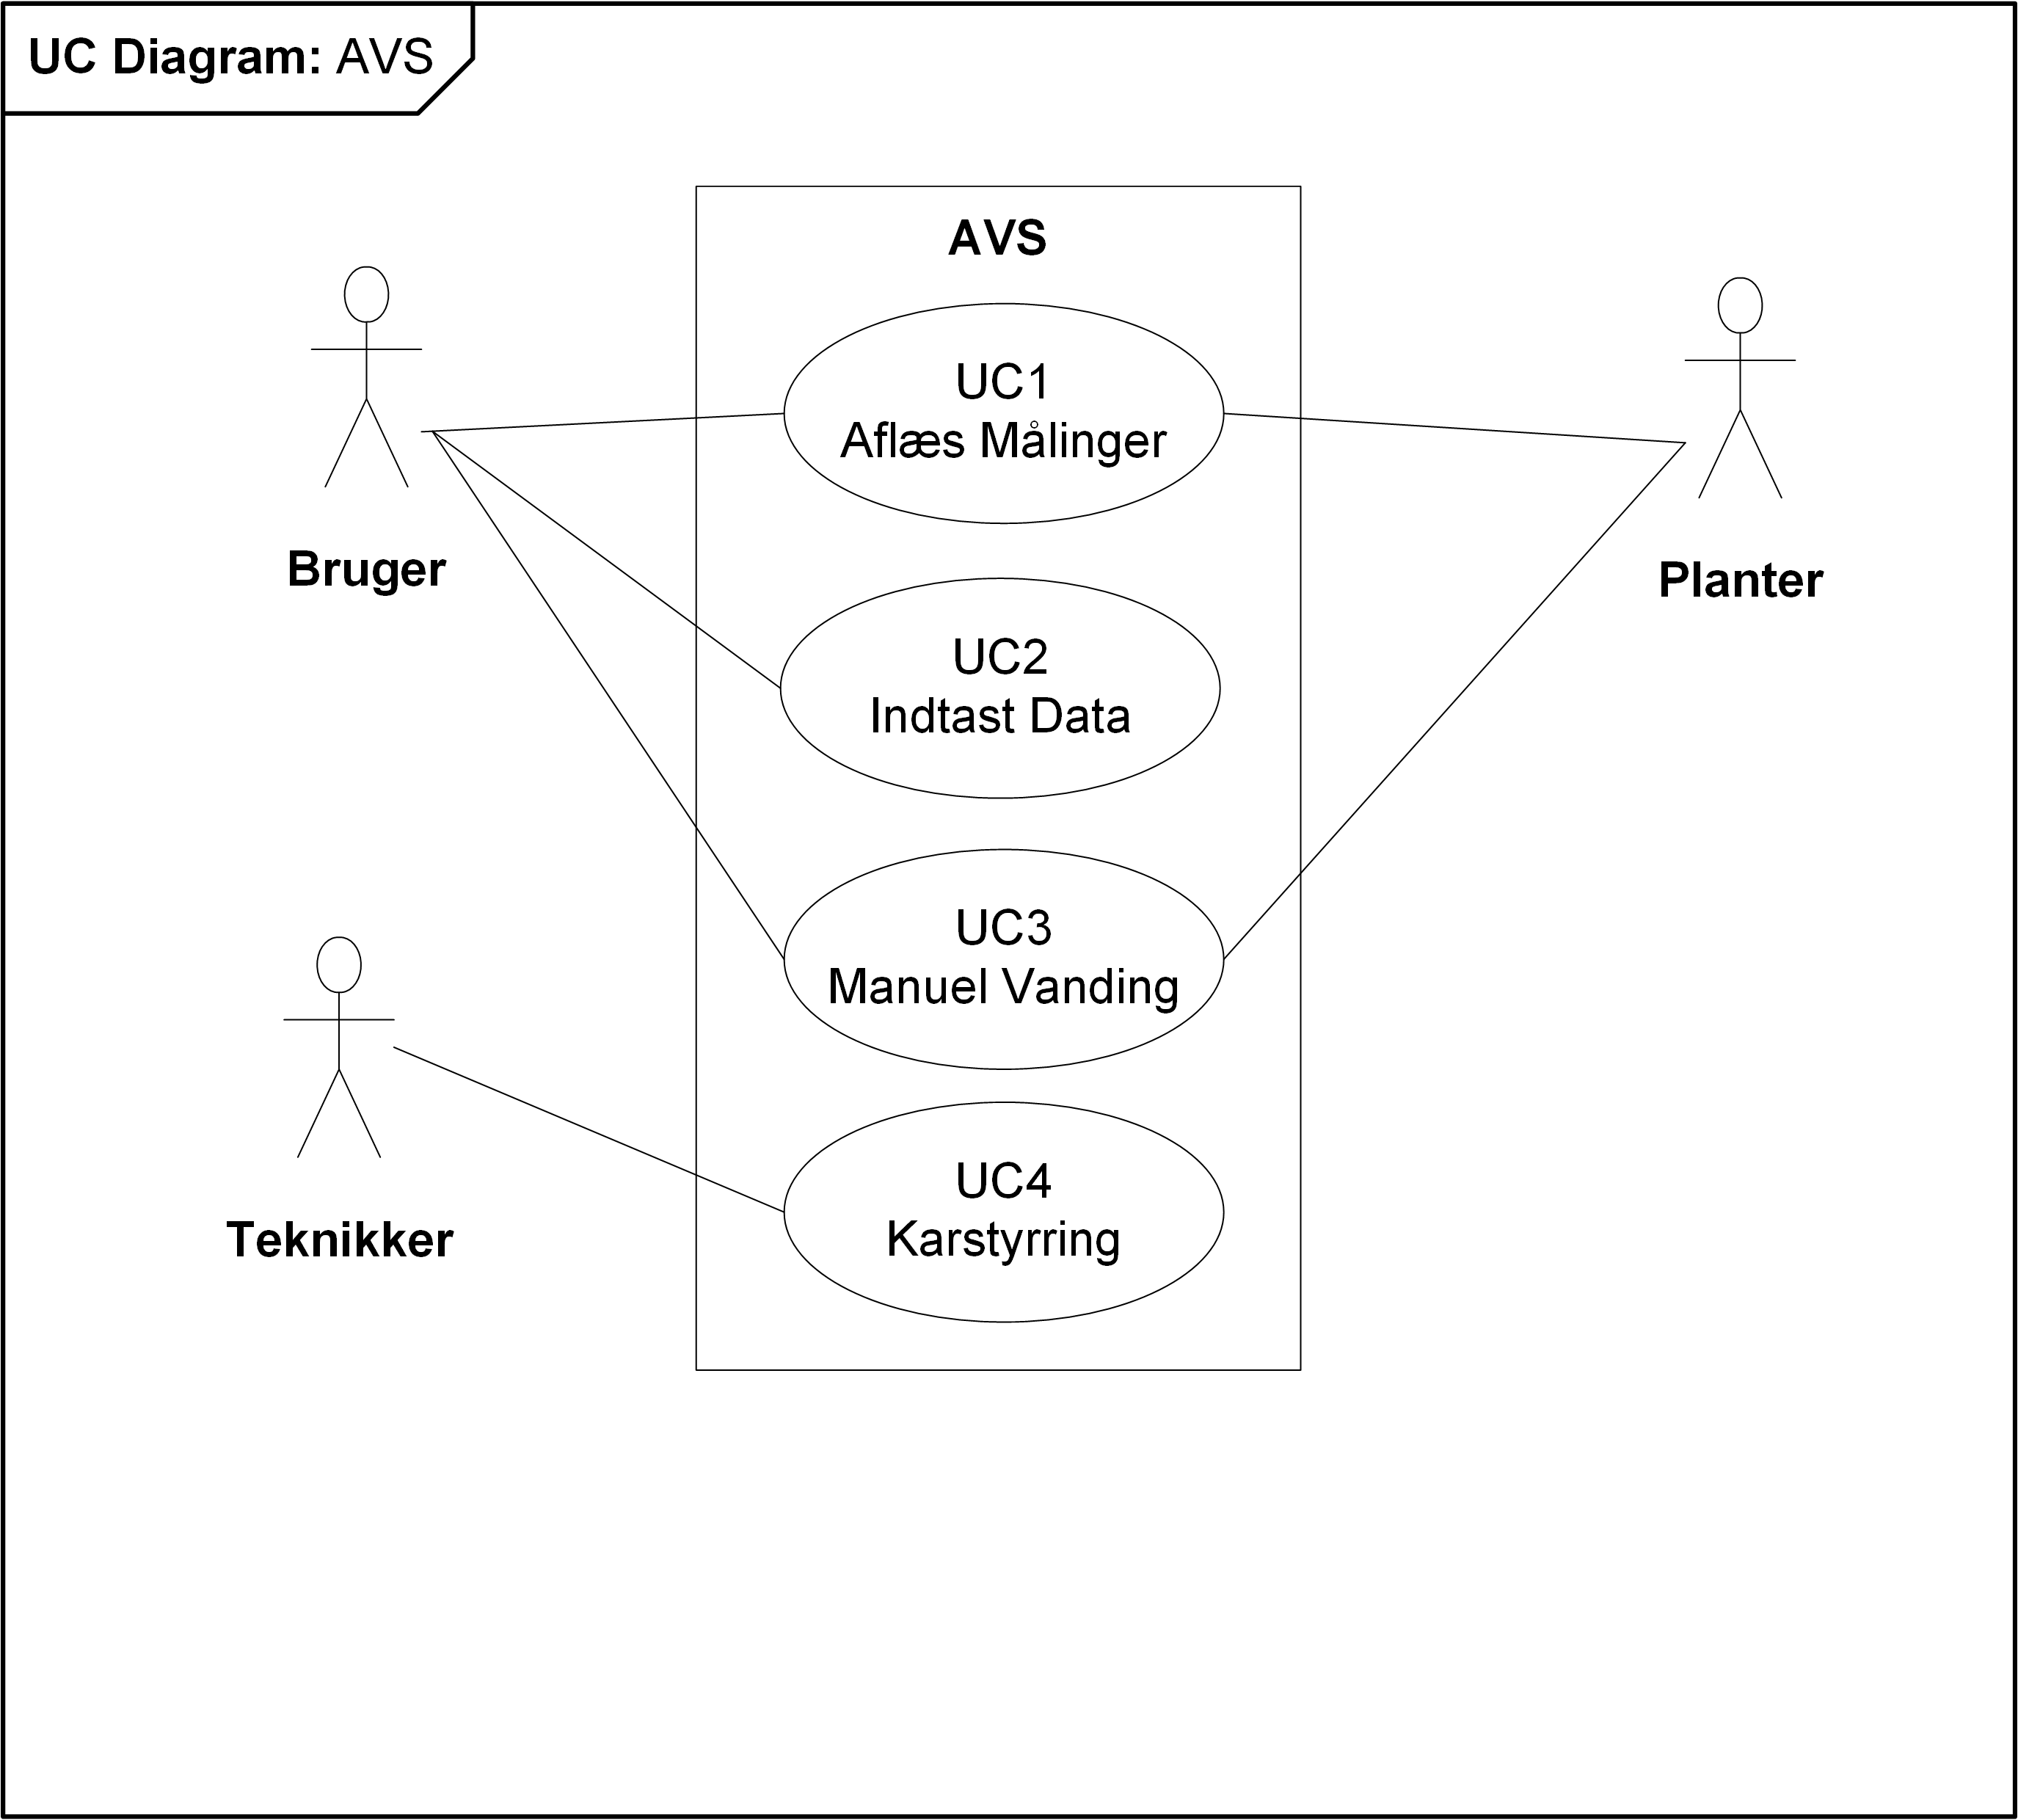
\includegraphics[scale=1]{Kravspecifikation/UseCases/Photo/AVS_UseCases}
	\caption{AVS Use case diagram}
	\label{photo:UseCD}
\end{figure}

\newpage
%	#1 Kalibrer pH-probe
\newpage
%!TEX root = ../../main.tex

\subsection*{Use case 1}
I denne use case kalibreres pH-proben, som er tilsluttet et kar. Dette skal gøres når systemet startes op. 
\begin{usecase}

\addtitle{Use Case 1}{Kalibrer pH-probe} 

\addfield{Mål:}{
	At kalibrere en pH-probe
}

\addfield{Initieret af:}{
	Tekniker   
}

\additemizedfield{Aktører:}{\item Primær: Tekniker}

\addfield{Samtidige forekomster:}{1}

%Preconditions: What must be true on start and worth telling the reader?
\addfield{Prækondition:}{ En rød LED lyser på karprintet og Teknikeren er i besiddelse af en buffer-væske med pH-værdi på 7}

%Postconditions: What must be true on successful completion and worth telling the reader
\addfield{Postkondition:}{pH-proben er kalibreret og en grøn LED lyser på karprintet\fxnote{glossary til karprint} tilhørende pH-proben }

%Main Success Scenario: A typical, unconditional happy path scenario of success.
\addscenario{Hovedscenarie:}{
	\item Tekniker sætter pH-proben ned i buffer-væsken
	\item Tekniker venter i 2 min 		
	\item Tekniker trykker på knappen \textit{kalibrer} i 3 sekunder
	\item Karprintet indlæser værdien fra proben
	\item Rød LED slukker
	\item Grøn LED lyser 			
}

%Extensions: Alternate scenarios of success or failure.
%\addscenario{Udvidelser:}{
%	\item[Ex.1] Teknikeren ønsker kun at aflæse værdier:
%		\begin{enumerate}
%		\item[1.] Teknikeren trykker på "OK"
%		\end{enumerate}
%}


\end{usecase}

%	#2 Opret kar
\newpage
\subsection*{Use case 2}
I denne use case opretter Tekniker et nyt kar. 
\begin{usecase}

\addtitle{Use Case 2}{Opret kar} 

\addfield{Mål:}{
At oprette et nyt kar i systemet
}

\addfield{Initieret af:}{
	Tekniker   
}

\additemizedfield{Aktører:}{\item Primær: Tekniker}

\addfield{Samtidige forekomster:}{1}

%Preconditions: What must be true on start and worth telling the reader?
\addfield{Prækondition:}{Ledig adresse på bussen i domæne 1}

%Postconditions: What must be true on successful completion and worth telling the reader
\addfield{Postkondition:}{Der er oprettet et kar}

%Main Success Scenario: A typical, unconditional happy path scenario of success.
\addscenario{Hovedscenarie:}{
	\item Tekniker trykker på \textit{Service} knappen i \glslink{gui}{gui'en}
	\item Systemet viser service menuen 
	\item Tekniker trykker på \textit{Opret kar} i service menu
	\item Systemet viser en menu hvor det er muligt at
	      indtaste navn og adresse til et nyt kar 
	\item Tekniker indtaster navn i feltet \textit{Navn}
	\item Tekniker indtaster \textit{Adresse} i feltet \textit{Adresse}
	\item Tekniker trykker \textit{Opret kar}
	\item Systemet opretter et nyt kar og sender Teknikeren til forsiden
	\item Det nye kar forekommer nu i hoved menuen
}

%Extensions: Alternate scenarios of success or failure.
%\addscenario{Udvidelser:}{
%	\item[Ex.1] Teknikeren ønsker kun at aflæse værdier:
%		\begin{enumerate}
%		\item[1.] Teknikeren trykker på "OK"
%		\end{enumerate}
%}


\end{usecase}

%	#3 Opret Sensor Ø
\newpage
%!TEX root = ../../main.tex

\subsection*{Use case 3}
I denne use case Oprettes en \gls{sensoroe}, den kan kun tilgås af Teknikeren, som er nødt til at kende adressen på sensor øen. 
\begin{usecase}

\addtitle{Use Case 3}{Opret Sensor Ø} 

\addfield{Mål:}{
At Oprette en Sensor Ø
}

\addfield{Initieret af:}{
	Tekniker   
}

\addfield{Aktører:}{Primær: Tekniker}

\addfield{Samtidige forekomster:}{1}

%Preconditions: What must be true on start and worth telling the reader?
\addfield{Prækondition:}{Teknikeren kender adressen til \glslink{sensoroe}{Sensor Øen}}

%Postconditions: What must be true on successful completion and worth telling the reader
\addfield{Postkondition:}{Der er oprettet en \gls{sensoroe} til det ønskede kar}

%Main Success Scenario: A typical, unconditional happy path scenario of success.
\addscenario{Hovedscenarie:}{
	\item Teknikeren sætter \glslink{sensoroe}{Sensor Øen} til kar bussen 
	\item Teknikeren trykker på det ønskede kar i \glslink{gui}{gui'en}
	\item Systemet viser et skærmbillede hvor det er muligt at oprette en sensor Ø
	\item Teknikeren trykker på \textit{Opret Sensorø}
	\item Systemet viser en menu hvor det er muligt at indtaste en adresse
	\item Teknikeren indtaster adresse i adresse feltet
	\item Teknikeren trykker \textit{Opret Sensorøen}
	\item Den nye \gls{sensoroe} forekommer nu i listen over \glslink{sensoroe}{Sensor Øer}. 
}

%Extensions: Alternate scenarios of success or failure.
%\addscenario{Udvidelser:}{
%	\item[Ex.1] Teknikeren ønsker kun at aflæse værdier:
%		\begin{enumerate}
%		\item[1.] Teknikeren trykker på "OK"
%		\end{enumerate}
%}


\end{usecase}
%	#4 Fyld kar
\newpage
%!TEX root = ../../main.tex

\subsection*{Use case 4}
I denne use case fyldes karet via indløbsventilen med vand. Indløbsventilen kan styres af Brugeren via guien.   
\begin{usecase}

\addtitle{Use Case 4}{Fyld kar} 

\addfield{Mål:}{
At fylde karet med vand
}

\addfield{Initieret af:}{
	Bruger  
}

\additemizedfield{Aktører:}{\item Primær: Bruger}

\addfield{Samtidige forekomster:}{1}

%Preconditions: What must be true on start and worth telling the reader?
\addfield{Prækondition:}{Karet er tomt}

%Postconditions: What must be true on successful completion and worth telling the reader
\addfield{Postkondition:}{Karet er fyldt med vand}

%Main Success Scenario: A typical, unconditional happy path scenario of success.
\addscenario{Hovedscenarie:}{
	\item Bruger trykker på det ønskede kar i \glslink{gui}{gui'en}
	\item Systemet viser et skærmbillede hvor man kan tilgå ventilstyringen
	\item Bruger trykker på \textit{Åben indløbsventil} 
	\item Indløbsventilen bliver åbnet og karet bliver fyldt med vand
	\item Når Brugeren ikke ønsker at fylde karet længere trykker Brugeren på \textit{Luk indløbsventil}
	\item Indløbsventilen bliver lukket og systemet stopper med at fylde karet med vand. 
}

%Extensions: Alternate scenarios of success or failure.
%\addscenario{Udvidelser:}{
%	\item[Ex.1] Teknikeren ønsker kun at aflæse værdier:
%		\begin{enumerate}
%		\item[1.] Teknikeren trykker på "OK"
%		\end{enumerate}
%}


\end{usecase}

%	#5 Indtast pH
\newpage
\subsection*{Use case 5}
I denne use case indtaster brugeren en pH-værdi, så den ønskede værdi kan ses. 
\begin{usecase}

\addtitle{Use Case 5}{Indtast pH-værdi} 

\addfield{Mål:}{
At indtaste og visualisere den ønskede pH-værdi
}

\addfield{Initieret af:}{
	Bruger   
}

\additemizedfield{Aktører:}{\item Primær: Bruger}

\addfield{Samtidige forekomster:}{1}

%Preconditions: What must be true on start and worth telling the reader?
\addfield{Prækondition:}{Et kar er oprettet og systemet er funktionelt}

%Postconditions: What must be true on successful completion and worth telling the reader
\addfield{Postkondition:}{Systemet opdaterer og visualisere den ønskede pH-værdi}

%Main Success Scenario: A typical, unconditional happy path scenario of success.
\addscenario{Hovedscenarie:}{
	\item Bruger trykker på det ønskede kar i \glslink{gui}{gui'en}
	\item Systemet viser et skærmbillede hvor det er muligt at indtaste en pH-værdi 	
	\item Bruger trykker på feltet uden for \textit{pH-Værdi} hvor der er en angivet værdi
	\item Bruger retter værdien til en ønskede pH-værdi
	\item Bruger trykker på \textit{Gem data}
	\item Systemet gemmer pH-værdien
}

%Extensions: Alternate scenarios of success or failure.
%\addscenario{Udvidelser:}{
%	\item[Ex.1] Teknikeren ønsker kun at aflæse værdier:
%		\begin{enumerate}
%		\item[1.] Teknikeren trykker på "OK"
%		\end{enumerate}
%}


\end{usecase}

%	#6 Indtast volumen
\newpage
\subsection*{Use case 6}
I denne use case indtaster Brugeren en volumen, så den ønskede værdi kan ses. 
\begin{usecase}

\addtitle{Use Case 6}{Indtast volumen} 

\addfield{Mål:}{
At indtaste og visualisere den ønskede volumen
}

\addfield{Initieret af:}{
	Bruger   
}

\addfield{Aktører:}{Primær: Bruger}

\addfield{Samtidige forekomster:}{1}

%Preconditions: What must be true on start and worth telling the reader?
\addfield{Prækondition:}{Et kar er oprettet og systemet er funktionelt}

%Postconditions: What must be true on successful completion and worth telling the reader
\addfield{Postkondition:}{Systemet opdaterer og visualisere den ønskede volumen}

%Main Success Scenario: A typical, unconditional happy path scenario of success.
\addscenario{Hovedscenarie:}{
	\item Bruger trykker på det ønskede kar i  \glslink{gui}{gui'en}
	\item Systemet viser et skærmbillede hvor det er muligt at indtaste en volumen
	\item Bruger trykker på feltet uden for \textit{volumen}, hvor der er en angivet værdi.
	\item Bruger retter værdien til en ønskede volumen i liter
	\item Bruger trykker på \textit{Gem data}
	\item Systemet gemmer volumen
}

%Extensions: Alternate scenarios of success or failure.
%\addscenario{Udvidelser:}{
%	\item[Ex.1] Teknikeren ønsker kun at aflæse værdier:
%		\begin{enumerate}
%		\item[1.] Teknikeren trykker på "OK"
%		\end{enumerate}
%}


\end{usecase}

%	#7 Aflæs målinger
\newpage
\subsection*{Use case 7}
Når Bruger ønsker at aflæse målingerne, kan personen tilgå de forskellige kar og aflæses data via \glslink{gui}{gui'en}.

\begin{usecase}

\addtitle{Use Case 7}{Aflæs målinger} 

\addfield{Mål:}{Bruger aflæser ønskede målinger}

\addfield{Initieret af:}{Bruger}

\addfield{Aktører:}{Primær: Bruger}

\addfield{Samtidige forekomster:}{1 }

%Preconditions: What must be true on start and worth telling the reader?
\addfield{Prækondition:}{Et fungerende system}

%Postconditions: What must be true on successful completion and worth telling the reader
\addfield{Postkondition:}{Målinger er aflæst af Bruger}

%Main Success Scenario: A typical, unconditional happy path scenario of success.
\addscenario{Hovedscenario:}{
	\item Bruger trykker på det ønskede kar i \glslink{gui}{gui'en}
	\item Systemet viser et skærmbillede med oversigt over kar data.
	\item Bruger aflæser de ønskede målinger.
}

%Extensions: Alternate scenarios of success or failure.
%\addscenario{Extensions:}{
%	\item[2.a] Invalid login data:
%		\begin{enumerate}
%		\item[1.] System shows failure message
%		\item[2.] User returns to step 1
%		\end{enumerate}
%	\item[5.a] Invalid subsriber data:
%		\begin{enumerate}
%		\item[1.] System shows failure message
%		\item[2.] User returns to step 2 and corrects the errors
%		\end{enumerate}
%}


\end{usecase}

%	#8 Manuel vanding
\newpage
\subsection*{Use case 8}
I denne use case ønsker Bruger at tilføre vand manuelt til planterne. For at denne use case kan gennemføres skal der være vand i det kar der ønskes at vande fra samt at dette er tilføjet til systemet. Karet skal være koblet på mindst en sensor ø.
\begin{usecase}

\addtitle{Use Case 8}{Manuel vanding} 

\addfield{Mål:}{At tilføre vand til planterne}

\additemizedfield{Initieret af:}{
	\item Bruger
}

\addfield{Aktører:}{Primær: Bruger}

\addfield{Samtidige forekomster:}{1}

%Preconditions: What must be true on start and worth telling the reader?
\addfield{Prækondition:}{Der skal være vand i det kar der ønskes at vande fra og der skal være tilkoblet mindst en sonsor ø. \glslink{gui}{gui'en} befinder sig i hovedmenuen}

%Postconditions: What must be true on successful completion and worth telling the reader
\addfield{Postkonditions:}{Der er vand ved planterne}

%Main Success Scenario: A typical, unconditional happy path scenario of success.
\addscenario{Hovedscenario:}{
	\item Bruger trykker på det ønskede kar i \glslink{gui}{gui'en}
	\item Systemet viser et skærmbillede hvor der kan vælges manuel vanding
	\item Bruger trykker på \textit{Start manuel vanding}
	\item Systemet begynder at vande
%	\item[ ] [Ex.1 Karret er tomt]
	\item Når der ikke ønskes at vande længere trykker Bruger på \textit{Stop manuel vanding}
	\item Systemet stopper med at vande
}

%Extensions: Alternate scenarios of success or failure.
%\addscenario{Udvidelser:}{
%	\item[Ex.1] Karret er tomt:
%		\begin{enumerate}
%		\item[1.] Systemet stopper med at vande
%		\end{enumerate}
%}


\end{usecase}

%	#9 Tøm kar
\newpage
%!TEX root = ../../main.tex

\subsection*{Use case 9}
I denne use case Tømmes karet via afløbsventilen. Afløbsventilen kan styres af Brugeren via \gls{gui}{gui'en}. 
\begin{usecase}

\addfield{Use Case 9}{Tøm kar} 

\additemizedfield{Mål:}{
\item At tømme karet for væske
}

\addfield{Initieret af:}{
	Bruger  
}

\addfield{Aktører:}{Primær: Bruger}

\addfield{Samtidige forekomster:}{1}

%Preconditions: What must be true on start and worth telling the reader?
\addfield{Prækondition:}{Karet indeholder vand}

%Postconditions: What must be true on successful completion and worth telling the reader
\addfield{Postkondition:}{Karet er tømt for væske}

%Main Success Scenario: A typical, unconditional happy path scenario of success.
\addscenario{Hovedscenarie:}{
	\item Systemet trykker på det ønskede kar i \glslink{gui}{gui'en}
	\item Systemet viser et skærmbillede hvor man kan tilgå ventilstyringen
	\item Bruger trykker på \textit{Åben afløbsventil} 
	\item Afløbsventilen bliver åbnet og karet bliver tømt for væske
	\item Når karet er tømt for vand trykker Brugeren på \textit{Luk afløbsventil}
	\item Afløbsventilen bliver lukket og karet er tom. 
}

%Extensions: Alternate scenarios of success or failure.
%\addscenario{Udvidelser:}{
%	\item[Ex.1] Teknikeren ønsker kun at aflæse værdier:
%		\begin{enumerate}
%		\item[1.] Teknikeren trykker på "OK"
%		\end{enumerate}
%}


\end{usecase}
%	#10 Slet kar
\newpage
\subsection*{Use case 10}
I denne use case sletter Tekniker et kar.
\begin{usecase}

\addtitle{Use Case 10}{Slet kar} 

\addfield{Mål:}{
At slette et kar i systemet
}

\addfield{Initieret af:}{
	Tekniker   
}

\additemizedfield{Aktører:}{\item Primær: Tekniker}

\addfield{Samtidige forekomster:}{1}

%Preconditions: What must be true on start and worth telling the reader?
\addfield{Prækondition:}{Der er oprettet mindst et kar i systemet}

%Postconditions: What must be true on successful completion and worth telling the reader
\addfield{Postkondition:}{Karet er slettet fra systemmet}

%Main Success Scenario: A typical, unconditional happy path scenario of success.
\addscenario{Hovedscenarie:}{
	\item Systemet viser en liste over oprettede kar, med en slet knap uden for hvert kar.
	\item Tekniker trykker på slet ud for det kar han ønsker at slette
	\item Systemet spørger om Teknikeren er sikker i en dialog
	\item Tekniker trykker \textit{ok}
	\item Systemet sletter karet
	\item Systemet returnerer Tekniker til listen over oprettede kar
}

%Extensions: Alternate scenarios of success or failure.
%\addscenario{Udvidelser:}{
%	\item[Ex.1] Teknikeren ønsker kun at aflæse værdier:
%		\begin{enumerate}
%		\item[1.] Teknikeren trykker på "OK"
%		\end{enumerate}
%}


\end{usecase}



%	#Ikke fully dressed Use cases
\newpage
\subsubsection{Use Case 8 - Skift vand}
I denne use case skal bruger/tekniker skifte vand i vandkaret. Dette kan skyldes at der skal tilsættes nyt gødning.

\subsubsection{Use Case 9 - Alarm}
Ved brugerdefineret grænseværdier (jordfugtighed og pH-værdi), afgiver systemet en alarm, f.eks. via. e-mail. 

\subsubsection{Use Case 10 - Ugeplan}
I denne use case får bruger mulighed for at indtaste en ugeplan for styring af dosering af gødning og vand til gromediet i løbet af ugen. 

\subsubsection{Use Case 11 - Udprint log}
Bruger kan få udprintet en log over de hændelser der er forekommet i systemet, bla. sensordata og dosering af vand.

%   #Ikke funktionelle krav
\newpage
\section{Ikke Funktionelle Krav}
Brugervenlighed:
\begin{itemize}
	\item Skal være intuitivt og let at opererer for udefrakommende:
	Der forudsettes en fungerende standard PC med Windows inkl. Explore/Chrome	/Firefox som browser

	\item Systemet skal kunne tilgås igennem en normal webbrowser:
		Her menes Explorer / Google Chrome / Firefox
	\item Systemet skal kunne tilgås over lokalt netværk samt over www
		Her forudsættes en fungerende internetopkoling og evt. lokalt netværk
\end{itemize}

Systembetingelser:
\begin{itemize}
	\item Systemet skal kunne fungere stabilt i temperaturintervallet (1 - 45grader Celsius)
	\item Systemet skal kunne fungere stabilt under høj luftfugtighed (op til 50%)
	\item Systemet skal være let at vedligeholde på daglig basis
		Systemets reservedele skal være lette at udskifte og skaffe.
\end{itemize}

Ydelse:
\begin{itemize}
	\item Systemet skal kunne fylde vandkarret på max. 2 min.
	\item Systemet skal kunne tømme vandkarret på max. 2 min.
	\item Systemet skal kunne dosere vand til gromediet med min 0,5 / max 2 liter/min.
	\item Systemet skal kunne dosere gødning til karret på max. 30 sek.
\end{itemize}

%	#Skitse over interface
%!TEX root = ../../main.tex
\section{Interface}
Interfacet (\gls{gui}'en) kan tilgås via en webbrowser som med udgangspunkt ligner Figur \ref{fig:index} og \ref{fig:kar}.
\begin{figure}[H]
    \centering
    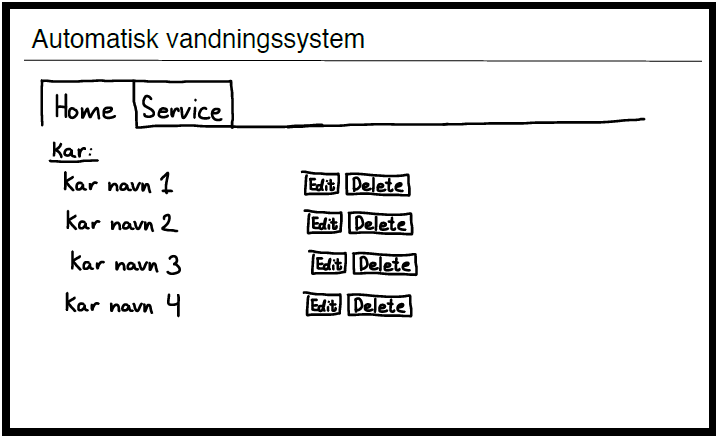
\includegraphics[width=0.7\textwidth]{Kravspecifikation/Interface/photo/index.PNG}
    \caption{AVS Interface - home}
    \label{fig:index}
\end{figure}
På Figur \ref{fig:index} kan brugeren se en liste over de kar der er oprettet, hvor de forskellige kar kan tilgås hvis brugeren klikker på det ønskede kar. 
\\\\
Under service har teknikeren mulighed for at oprette et \gls{kar}, hvor han indtaster adresse, navn og derefter trykker opret \gls{kar}. hvorefter karet kommer frem på listen over \gls{kar}. ydermere er der en delete og edit knap uden for hvert \gls{kar} så teknikeren har mulighed for at slette et \gls{kar} eller redigerer navnet. 
\\\\
Når brugeren trykker på et \gls{kar} tilgår han/hun et interface for \gls{kar}et, som kan ses på Figur \ref{fig:kar}. 
\begin{figure}[H]
    \centering
    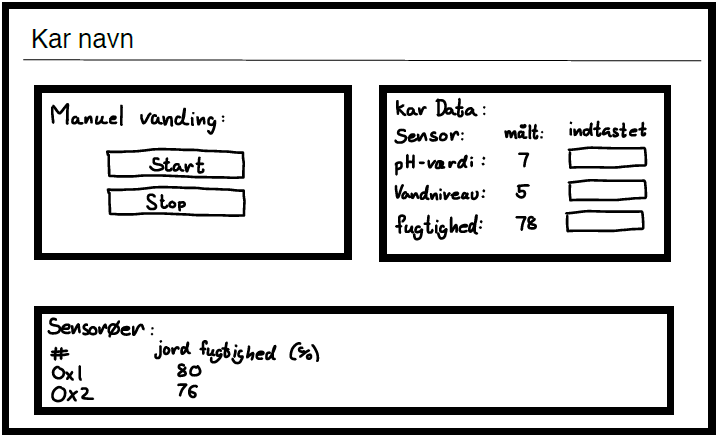
\includegraphics[width=0.7\textwidth]{Kravspecifikation/Interface/photo/kar.PNG}
    \caption{AVS Interface - kar}
    \label{fig:kar}
\end{figure}

I feltet øverste til venstre er der mulighed for manuel vanding, hvor brugeren trykker på start når han/hun vil starte den manuelle vanding. For at stoppe den manuelle vanding trykke på bruger på stop.   
\\\\
I feltet øverst til højre har brugeren mulighed for at indtaste de ønskede data og aflæse de data der kommer fra de forskellige sensor. 
\\\\
I det nederste felt kan der ses en liste over \gls{sensoroe}erne hvor brugeren kan aflæse de data der kommer fra de forskellige sensor.   
